\documentclass[]{article}
\usepackage{lmodern}
\usepackage{amssymb,amsmath}
\usepackage{ifxetex,ifluatex}
\usepackage{fixltx2e} % provides \textsubscript
\ifnum 0\ifxetex 1\fi\ifluatex 1\fi=0 % if pdftex
  \usepackage[T1]{fontenc}
  \usepackage[utf8]{inputenc}
\else % if luatex or xelatex
  \ifxetex
    \usepackage{mathspec}
  \else
    \usepackage{fontspec}
  \fi
  \defaultfontfeatures{Ligatures=TeX,Scale=MatchLowercase}
\fi
% use upquote if available, for straight quotes in verbatim environments
\IfFileExists{upquote.sty}{\usepackage{upquote}}{}
% use microtype if available
\IfFileExists{microtype.sty}{%
\usepackage{microtype}
\UseMicrotypeSet[protrusion]{basicmath} % disable protrusion for tt fonts
}{}
\usepackage[margin=1in]{geometry}
\usepackage{hyperref}
\hypersetup{unicode=true,
            pdftitle={Temperature dependence of biomass and ecosystem function depend on species interactions. Supplementary File 2: Phytoplankton and oxygen flux results in main text.},
            pdfborder={0 0 0},
            breaklinks=true}
\urlstyle{same}  % don't use monospace font for urls
\usepackage{longtable,booktabs}
\usepackage{graphicx,grffile}
\makeatletter
\def\maxwidth{\ifdim\Gin@nat@width>\linewidth\linewidth\else\Gin@nat@width\fi}
\def\maxheight{\ifdim\Gin@nat@height>\textheight\textheight\else\Gin@nat@height\fi}
\makeatother
% Scale images if necessary, so that they will not overflow the page
% margins by default, and it is still possible to overwrite the defaults
% using explicit options in \includegraphics[width, height, ...]{}
\setkeys{Gin}{width=\maxwidth,height=\maxheight,keepaspectratio}
\IfFileExists{parskip.sty}{%
\usepackage{parskip}
}{% else
\setlength{\parindent}{0pt}
\setlength{\parskip}{6pt plus 2pt minus 1pt}
}
\setlength{\emergencystretch}{3em}  % prevent overfull lines
\providecommand{\tightlist}{%
  \setlength{\itemsep}{0pt}\setlength{\parskip}{0pt}}
\setcounter{secnumdepth}{0}
% Redefines (sub)paragraphs to behave more like sections
\ifx\paragraph\undefined\else
\let\oldparagraph\paragraph
\renewcommand{\paragraph}[1]{\oldparagraph{#1}\mbox{}}
\fi
\ifx\subparagraph\undefined\else
\let\oldsubparagraph\subparagraph
\renewcommand{\subparagraph}[1]{\oldsubparagraph{#1}\mbox{}}
\fi

%%% Use protect on footnotes to avoid problems with footnotes in titles
\let\rmarkdownfootnote\footnote%
\def\footnote{\protect\rmarkdownfootnote}

%%% Change title format to be more compact
\usepackage{titling}

% Create subtitle command for use in maketitle
\newcommand{\subtitle}[1]{
  \posttitle{
    \begin{center}\large#1\end{center}
    }
}

\setlength{\droptitle}{-2em}

  \title{Temperature dependence of biomass and ecosystem function depend on
species interactions. Supplementary File 2: Phytoplankton and oxygen
flux results in main text.}
    \pretitle{\vspace{\droptitle}\centering\huge}
  \posttitle{\par}
    \author{}
    \preauthor{}\postauthor{}
    \date{}
    \predate{}\postdate{}
  

\begin{document}
\maketitle

\#\#. temporal results
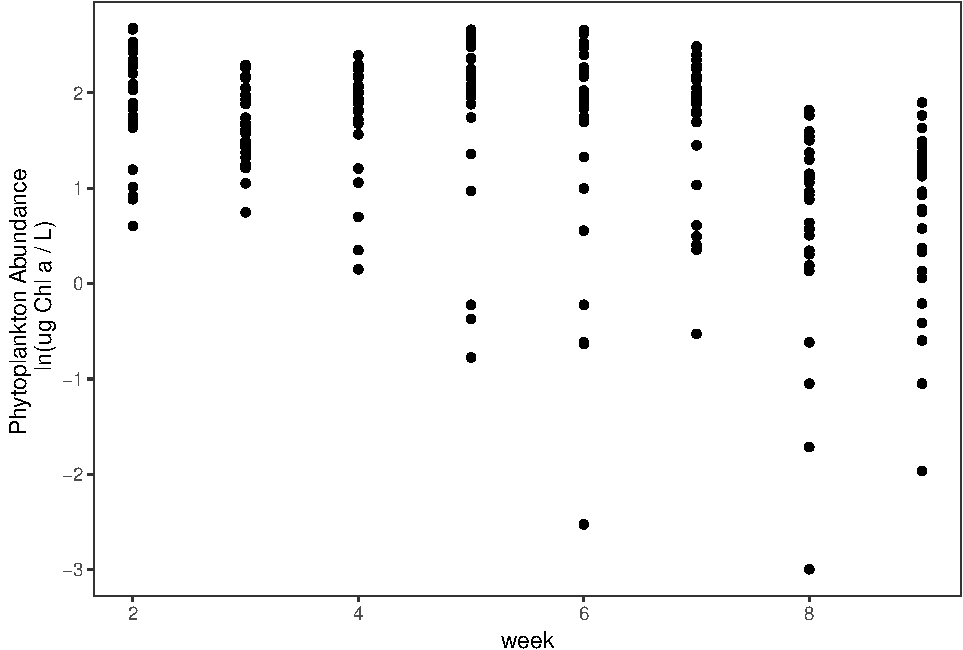
\includegraphics{Garzke_markdown_files/figure-latex/unnamed-chunk-2-1.pdf}

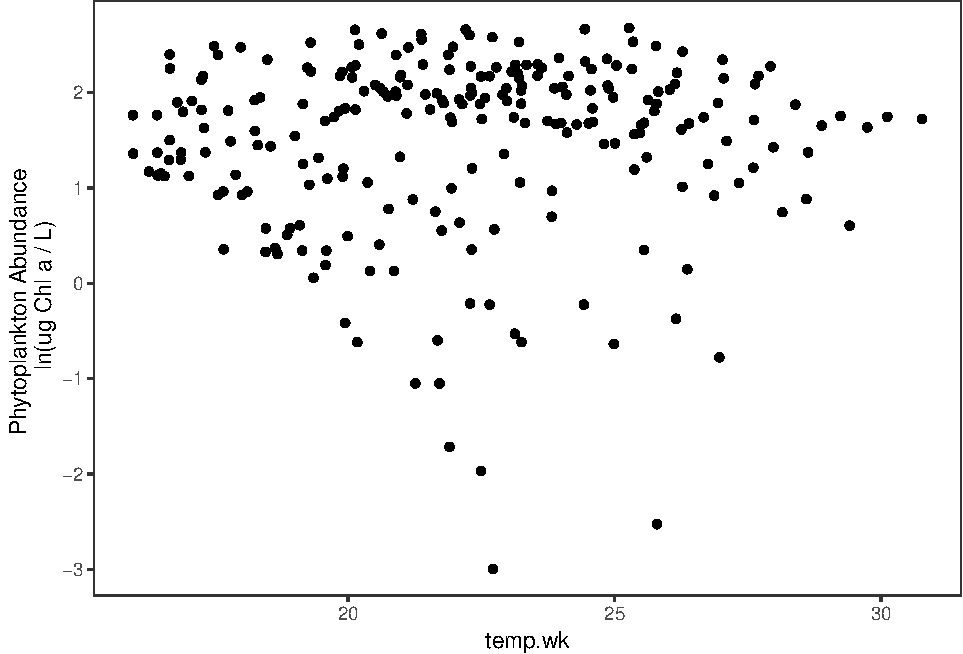
\includegraphics{Garzke_markdown_files/figure-latex/unnamed-chunk-3-1.pdf}

\subsection{1. Trophic Cascade Results (Figure 2 Main
text)}\label{trophic-cascade-results-figure-2-main-text}

Figure S2. 2: Trophic Treatment Effects on Chlorophyll a, Net Oxygen
Ecosystem Production (NEP), and Net Ecosystem Respiration (ER)

\begin{verbatim}
## TableGrob (1 x 3) "arrange": 3 grobs
##   z     cells    name           grob
## 1 1 (1-1,1-1) arrange gtable[layout]
## 2 2 (1-1,2-2) arrange gtable[layout]
## 3 3 (1-1,3-3) arrange gtable[layout]
\end{verbatim}

\subsubsection{2.1 Phytoplankton abundance (for Figure 3, Table 2 main
text)}\label{phytoplankton-abundance-for-figure-3-table-2-main-text}

Figure S2. 1: Chlorophyll a concentration

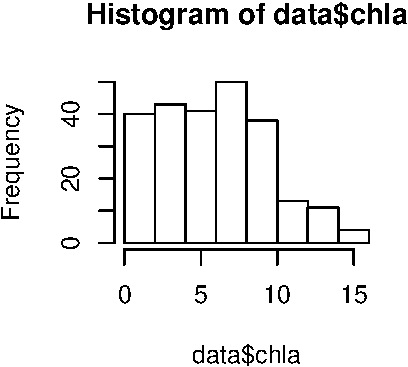
\includegraphics{Garzke_markdown_files/figure-latex/Fig_S2.1-1.pdf}
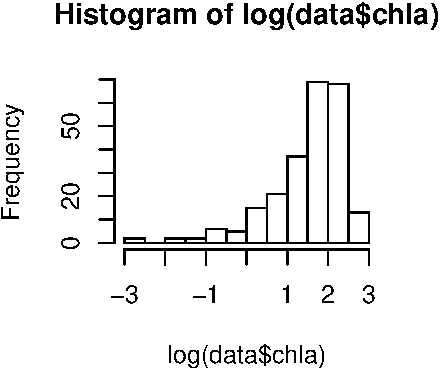
\includegraphics{Garzke_markdown_files/figure-latex/Fig_S2.1-2.pdf}

\subsection{2.1.1 Phytoplankton abundance candidate
models}\label{phytoplankton-abundance-candidate-models}

Table S2. 1: Model selection results for Phytoplankton (Chl a) for
linear mixed effects model

\begin{longtable}[]{@{}lrlrrrllrrrrr@{}}
\toprule
& Int & TL & Tw & Tt & Tw*Tt & Tw*TL & Tt*TL & df & logLik & AICc & d &
w\tabularnewline
\midrule
\endhead
modPB8 & 2.05 & + & -0.66 & 1.30 & NA & + & + & 11 & -162.86 & 348.87 &
0.00 & 9.528923e-01\tabularnewline
modPB7 & 2.05 & + & -0.96 & 1.30 & NA & NA & + & 9 & -168.05 & 354.89 &
6.02 & 4.698179e-02\tabularnewline
modPBF & 2.14 & + & -0.52 & 2.16 & 1.34 & + & NA & 10 & -172.89 & 366.74
& 17.86 & 1.259313e-04\tabularnewline
modPB4 & 1.50 & NA & -0.96 & 1.70 & 0.96 & NA & NA & 6 & -207.95 &
428.26 & 79.38 & 5.511062e-18\tabularnewline
modPB6 & 1.91 & + & -0.66 & NA & NA & + & NA & 8 & -206.58 & 429.79 &
80.92 & 2.557666e-18\tabularnewline
modPB3 & 1.50 & NA & -0.96 & 1.71 & NA & NA & NA & 5 & -211.74 & 433.74
& 84.86 & 3.556642e-19\tabularnewline
modPB5 & 1.91 & + & -0.96 & NA & NA & NA & NA & 6 & -211.45 & 435.27 &
86.40 & 1.653514e-19\tabularnewline
modPB2 & 1.50 & NA & -0.96 & NA & NA & NA & NA & 4 & -218.40 & 444.98 &
96.11 & 1.286913e-21\tabularnewline
modPB1 & 1.90 & + & NA & NA & NA & NA & NA & 5 & -257.21 & 524.68 &
175.81 & 6.345675e-39\tabularnewline
modPB0 & 1.49 & NA & NA & NA & NA & NA & NA & 3 & -264.15 & 534.41 &
185.54 & 4.902314e-41\tabularnewline
\bottomrule
\end{longtable}

Table S2. 2: Parameter estimates from model PB8 (Table S2.1) for
Phytoplankton (Chl a) for linear mixed effects model

\begin{longtable}[]{@{}lrrr@{}}
\toprule
& Ea & lower & upper\tabularnewline
\midrule
\endhead
P & 1.30 & 0.85 & 1.76\tabularnewline
PZ & 3.15 & 2.76 & 3.54\tabularnewline
PZN & 1.65 & 1.19 & 2.10\tabularnewline
\bottomrule
\end{longtable}

\section{}\label{section}

\subsection{2.2 Net ecosystem oxygen
production}\label{net-ecosystem-oxygen-production}

\includegraphics{Garzke_markdown_files/figure-latex/unnamed-chunk-10-1.pdf}
\includegraphics{Garzke_markdown_files/figure-latex/unnamed-chunk-10-2.pdf}

Table S2. 3: Model selection results for Net Ecosystem Oxygen
Production, with 1\textbar{}Tank as a random effect. Model terms are:
intercept (Int), trophic treatment (TL), Temperature - weekly average
(Tw), temperature - expt average (Tt), interaction terms and statistical
estimates

\begin{longtable}[]{@{}lrlrrrllrrrrr@{}}
\toprule
& Int & TL & Tw & Tt & Tw*Tt & Tw*TL & Tt*TL & df & logLik & AICc & d &
w\tabularnewline
\midrule
\endhead
modNPP8 & -6.42 & + & 0.29 & -1.41 & NA & + & + & 11 & -266.46 & 556.20
& 0.00 & 3.880444e-01\tabularnewline
modNPPF & -6.42 & + & 0.37 & -1.42 & 0.84 & + & + & 12 & -265.54 &
556.59 & 0.39 & 3.199070e-01\tabularnewline
modNPP7 & -6.41 & + & 0.03 & -1.39 & NA & NA & + & 9 & -269.68 & 558.21
& 2.01 & 1.421772e-01\tabularnewline
modNPP3 & -6.15 & NA & 0.02 & -0.96 & NA & NA & NA & 5 & -274.37 &
559.02 & 2.81 & 9.506575e-02\tabularnewline
modNPP4 & -6.15 & NA & 0.02 & -0.96 & 0.61 & NA & NA & 6 & -273.87 &
560.13 & 3.92 & 5.458021e-02\tabularnewline
modNPP0 & -6.15 & NA & NA & NA & NA & NA & NA & 3 & -283.15 & 572.41 &
16.20 & 1.177095e-04\tabularnewline
modNPP2 & -6.15 & NA & 0.03 & NA & NA & NA & NA & 4 & -283.13 & 574.44 &
18.24 & 4.256459e-05\tabularnewline
modNPP1 & -6.26 & + & NA & NA & NA & NA & NA & 5 & -282.25 & 574.78 &
18.58 & 3.589977e-05\tabularnewline
modNPP6 & -6.26 & + & 0.27 & NA & NA & + & NA & 8 & -279.83 & 576.34 &
20.14 & 1.642404e-05\tabularnewline
modNPP5 & -6.26 & + & 0.03 & NA & NA & NA & NA & 6 & -282.23 & 576.85 &
20.65 & 1.275902e-05\tabularnewline
\bottomrule
\end{longtable}

\paragraph{NPP Coefficients}\label{npp-coefficients}

Table S2. 4: Parameter estimates from model NPP8 (Table S2.3) for Net
Ecosystem Oxygen Productivity (NEP) for linear mixed effects model(For
MS Figure 3)

\begin{longtable}[]{@{}lrrr@{}}
\toprule
& Ea & lower & upper\tabularnewline
\midrule
\endhead
P & -1.41 & -2.25 & -0.58\tabularnewline
PZ & -1.21 & -2.36 & -0.07\tabularnewline
PZN & -0.99 & -2.10 & 0.12\tabularnewline
\bottomrule
\end{longtable}

\subparagraph{2.2 Net ecosystem oxygen consumption
(ER)}\label{net-ecosystem-oxygen-consumption-er}

\includegraphics{Garzke_markdown_files/figure-latex/Table_2.3-1.pdf}
\includegraphics{Garzke_markdown_files/figure-latex/Table_2.3-2.pdf}

Table S2. 5: Model selection results for Net Ecosystem Respiration, with
1\textbar{}Tank as a random effect. Model terms are: intercept (Int),
trophic treatment (TL), Temperature - weekly average (Tw), temperature -
expt average (Tt), interaction terms and statistical estimates

\begin{longtable}[]{@{}lrlrrrllrrrrr@{}}
\toprule
& Int & TL & Tw & Tt & Tw*Tt & Tw*TL & Tt*TL & df & logLik & AICc & d &
w\tabularnewline
\midrule
\endhead
modER7 & -6.03 & + & 0.26 & -1.32 & NA & NA & + & 9 & -158.72 & 336.33 &
0.00 & 8.117512e-01\tabularnewline
modER8 & -6.03 & + & 0.19 & -1.32 & NA & + & + & 11 & -158.19 & 339.72 &
3.39 & 1.492212e-01\tabularnewline
modERF & -5.98 & + & 0.25 & -0.81 & 0.57 & + & NA & 10 & -160.65 &
342.41 & 6.08 & 3.885201e-02\tabularnewline
modER3 & -5.74 & NA & 0.26 & -0.68 & NA & NA & NA & 5 & -172.34 & 354.98
& 18.64 & 7.257027e-05\tabularnewline
modER4 & -5.74 & NA & 0.26 & -0.64 & 0.60 & NA & NA & 6 & -171.28 &
354.98 & 18.65 & 7.255858e-05\tabularnewline
modER5 & -5.89 & + & 0.26 & NA & NA & NA & NA & 6 & -172.51 & 357.43 &
21.09 & 2.134098e-05\tabularnewline
modER6 & -5.89 & + & 0.19 & NA & NA & + & NA & 8 & -172.00 & 360.71 &
24.38 & 4.134606e-06\tabularnewline
modER1 & -5.90 & + & NA & NA & NA & NA & NA & 5 & -175.56 & 361.42 &
25.09 & 2.892592e-06\tabularnewline
modER2 & -5.74 & NA & 0.26 & NA & NA & NA & NA & 4 & -177.02 & 362.24 &
25.90 & 1.927201e-06\tabularnewline
modER0 & -5.76 & NA & NA & NA & NA & NA & NA & 3 & -180.12 & 366.35 &
30.02 & 2.461395e-07\tabularnewline
\bottomrule
\end{longtable}

\subsection{ER coefficients}\label{er-coefficients}

Table S2. 6: Confidence intervals for model ER7 (Table S2.5) (For MS
Figure 3

\begin{longtable}[]{@{}lrrr@{}}
\toprule
& Ea & lower & upper\tabularnewline
\midrule
\endhead
P & -1.3163396 & -1.8455347 & -0.7871445\tabularnewline
PZ & -0.8777488 & -1.3246951 & -0.4308026\tabularnewline
PZN & -0.3295142 & -0.8562013 & 0.1971728\tabularnewline
\bottomrule
\end{longtable}

\subparagraph{Figure 3 (Full)}\label{figure-3-full}

Figure S2. 3: Manuscript figure 3: Effects of temperature on oxygen flux
and phytoplankton standing stock

\includegraphics{Garzke_markdown_files/figure-latex/Fig_2.3-1.pdf}

\begin{verbatim}
## pdf 
##   2
\end{verbatim}


\end{document}
